\documentclass[journal,12pt,onecolumn]{IEEEtran}
\usepackage{graphicx, float}
\graphicspath{{Figs/}}
\usepackage{multicol}
\usepackage{parskip}
\usepackage{titlesec}
\usepackage{color}
\usepackage{enumitem}
\usepackage{amsmath,amssymb,amsfonts,amsthm}
\usepackage{array}
\usepackage{booktabs}
\usepackage[table]{xcolor}
\usepackage{longtable}
\usepackage{gensymb}
\usepackage{cite}
\usepackage{algorithmic}
\usepackage{textcomp}
\usepackage{txfonts}
\usepackage{listings}
\usepackage{mathtools}
\usepackage{comment}
\usepackage{tkz-euclide}
\usepackage[breaklinks=true]{hyperref}
\usepackage{gvv}
\usepackage[latin1]{inputenc}
\usetikzlibrary{arrows.meta, positioning}
\usepackage{xparse}
\usepackage{calc}
\usepackage{multirow}
\usepackage{hhline}
\usepackage{ifthen}
\usepackage{lscape}
\usepackage{tabularx}
\usepackage{circuitikz}
\usepackage{tikz}
\newtheorem{problem}{Problem}
\newtheorem{theorem}{Theorem}[section]
\newtheorem{proposition}{Proposition}[section]
\newtheorem{lemma}{Lemma}[section]
\newtheorem{corollary}[theorem]{Corollary}
\newtheorem{example}{Example}[section]
\newtheorem{definition}[problem]{Definition}
\newcommand{\BEQA}{\begin{eqnarray}}
\newcommand{\EEQA}{\end{eqnarray}}
\theoremstyle{remark}
\title{GATE EY 2015}
\author{AI25BTECH11016-VARUN}
\begin{document}
\maketitle

\textbf{Q.1 to Q.5 carry one mark each and Q.6 to Q.10 carry 2 marks each}
\begin{enumerate}
%1
 \item 
Choose the most appropriate word from the options given below to complete the following sentence:
The principal presented the chief guest with a  \underline{\hspace{1.5cm}},as token of appreciation.
\begin{multicols}{4}
\begin{enumerate}
    
\item momento
\item memento
\item momentum
\item moment

    \end{enumerate}
    \end{multicols}
\hfill{(GATE EY 2015)}
%2
\item Choose the appropriate word/phrase, out of the four options given below, to complete the following sentence:

Frogs  \underline{\hspace{1.5cm}}.

\begin{multicols}{4}
\begin{enumerate}
    
\item croak
\item roar
\item hiss
\item patter

    \end{enumerate}
    \end{multicols}
\hfill{(GATE EY 2015)}

\item 
Choose the word most similar in meaning to the given word:

Educe

\begin{multicols}{4}
\begin{enumerate}
    
\item Exert
\item Educate
\item Extract
\item Extend

    \end{enumerate}
    \end{multicols}
\hfill{(GATE EY 2015)}
%4
\item 

Operators $\Box$,$\Diamond$ and $\rightarrow$ are defined by: a$\Diamond$b = a+b/a-b;a$\Box$b=a-b/a+b;a$\rightarrow$b=ab.
Find the value of (66$\Box$6)$\rightarrow$(66$\Diamond$6)

\begin{multicols}{4}
\begin{enumerate}
    
\item -2
\item -1
\item  1
\item 2

    \end{enumerate}
    \end{multicols}
\hfill{(GATE EY 2015)}


%5
\item 
If $logx (5/7) = -1/3$, then the value of x is

\begin{multicols}{4}
\begin{enumerate}
    
\item 343/125
\item 125/343
\item -25/49
\item -49/25

    \end{enumerate}
    \end{multicols}
\hfill{(GATE EY 2015)}

%6
\item 
The following question presents a sentence, part of which is underlined.
Beneath the sentence you find four ways of phrasing the underlined part.
Following the requirements of standard written English, select the answer that produces the most effective sentence.

Tuberculosis, together with its effects, rank one of the leading causes of death in India.


\begin{enumerate}
    
\item ranks one of the leading causes of death
\item ranks as one of the leading causes of death
\item are the rank of one of the leading causes of death
\item are one of the leading causes of death

    \end{enumerate}
  
\hfill{(GATE EY 2015)}
%7
\item
Read the following paragraph and chose the correct statement.


Climate change has reduced human security and threatened human well being. An ignored reality of human progress is that human security largely depends upon environmental security. But on the contrary, human progress seems contradictory to environmental security. Ways to keep both the required in a given challenge is to address to one and all. One of the ways to curb the climate change may be via small scientific innovations, while the older may be the Gandhian perspective on small scale progress but with focus on sustainability.


\begin{enumerate}
    
\item Human progress and security are positively associated with environmental security.
\item  Human progress is contradictory to environmental security
\item Human security is contradictory to environmental security.
\item Human progress depends upon environmental security.



    \end{enumerate}
    
\hfill{(GATE EY 2015)}
%8
\item 
Fill in the missing value

\begin{figure}[H]
    \centering
    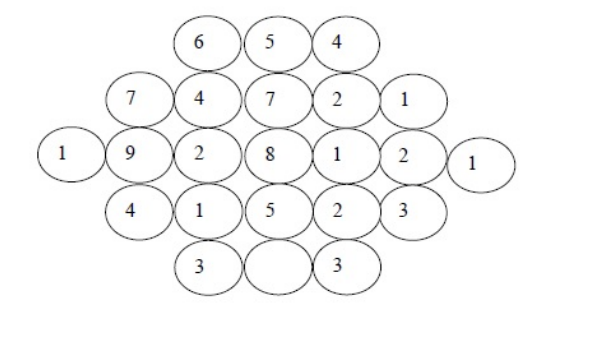
\includegraphics[]{figs/Q.8.png}
    \caption{}
    \label{fig:1}
\end{figure}

    
\hfill{(GATE EY 2015)}

%9
\item A cube of side 3 units is formed using a set of smaller cubes of side 1 unit.
Find the proportion of the number of faces of the smaller cubes visible to those which are NOT visible.


\begin{multicols}{4}
\begin{enumerate}
    
\item 1 : 4
\item 1 : 3
\item 1 : 2
\item 2 : 3

    \end{enumerate}
    \end{multicols}
\hfill{(GATE EY 2015)}


%10
\item Humpty Dumpty sits on a wall every day while having lunch. The wall sometimes breaks.
A person sitting on the wall falls if the wall breaks.

Which one of the statements below is logically valid and can be inferred from the above sentences?



\begin{enumerate}
    
\item Humpty Dumpty always falls while having lunch
\item Humpty Dumpty does not fall sometimes while having lunch
\item Humpty Dumpty never falls during dinner
\item When Humpty Dumpty does not sit on the wall, the wall does not break



    \end{enumerate}
    
\hfill{(GATE EY 2015)}
\textbf{Q.11 to Q.35 carry 1 mark each and Q.36 to Q.65 carry two marks each}

%11
\item 
A genetic locus has only two alleles in a population. The frequency of heterozygotes at this population is 0.32. Assuming Hardy-Weinberg equilibrium, the frequency (in decimal notation, not in fractions or percentage) of the rarer allele is \underline{\hspace{1.5cm}}


\hfill{(GATE EY 2015)}

%12
\item 

in a population of asexual organisms that remains at a constant size, an individual is expected to have an average of \underline{\hspace{1.5cm}}reproducing offspring.

\hfill{(GATE EY 2015)}

%13
\item 
Which of the following processes captures the KEY DIFFERENCE between metapopulation versus single-population approaches to study population dynamics?

\begin{multicols}{2}
\begin{enumerate}
    
\item  Births and Deaths
\item  Life history variation
\item Immigration and Emigration
\item Environmental and demographic stochasticity

    \end{enumerate}
    \end{multicols}
\hfill{(GATE EY 2015)}

%14

\item 
A researcher used a t-test on two samples of data and obtained the following statistics: sample t-statistic = 5.2, critical t-statistic = 2.3 (for the appropriate degrees of freedom and alpha level of 0.05). Based on this information, the researcher should conclude that


\begin{enumerate}
    
\item p $<$ 0.05, reject the statistical null hypothesis
\item p $<$ 0.05, fail to reject the statistical null hypothesis
\item p $>$ 0.05, reject the statistical null hypothesis
\item p $>$ 0.05, fail to reject the statistical null hypothesis

    \end{enumerate}
    
\hfill{(GATE EY 2015)}


%15

\item Among forests of the following states, tree diversity (e.g., species richness per unit area) is high in:


\begin{multicols}{4}
\begin{enumerate}
    
\item  P and Q
\item  Q and S
\item R and S
\item P and R

    \end{enumerate}
    \end{multicols}
\hfill{(GATE EY 2015)}

%16
\item 
Many agriculturally important plants belong to which of the following families?

P) Dipterocarpaceae, Q) Poaceae, R) Solanaceae, S) Verbenaceae

\begin{multicols}{4}
\begin{enumerate}
    
\item P and Q
\item Q and S
\item P and S 
\item Q and R

    \end{enumerate}
    \end{multicols}
\hfill{(GATE EY 2015)}
%17
\item 
In India, $Parthenium hysterophorus$, $Lantana camara$, and $Prosopis juliflora$ are examples of which of the following types of species?
P) Endangered species, Q) Endemic species, R) Invasive species, S) Keystone species

\begin{multicols}{4}
\begin{enumerate}
    
\item P only
\item P and Q
\item R only
\item S only

    \end{enumerate}
    \end{multicols}
\hfill{(GATE EY 2015)}

%18
\item 
Acid rain can be attributed to which of the following factors?

P) human alteration of global S cycle
Q) human alteration of global N cycle
R) increased average global temperature
S) natural causes such as fluctuation in sunspots
T) natural causes such as volcanism


\begin{multicols}{2}
\begin{enumerate}
    
\item P, Q, and R
\item P and R
\item S and T
\item P, Q, and T

    \end{enumerate}
    \end{multicols}
\hfill{(GATE EY 2015)}
%19
\item 
Periodic glaciation at a global scale is a feature of which geological age?

\begin{multicols}{4}
\begin{enumerate}
    
\item Cenozoic
\item Paleozoic
\item Jurassic
\item Archaean

    \end{enumerate}
    \end{multicols}
\hfill{(GATE EY 2015)}

\item Carbon-fixation reactions using RUBISCO and PEP occur in


\begin{multicols}{2}
\begin{enumerate}
    
\item C3 plants
\item C4 plants
\item CAM plants
\item C3, C4, and CAM plants

    \end{enumerate}
    \end{multicols}
\hfill{(GATE EY 2015)}
%21
\item 
Which of the following trees is phylogenetically MOST accurate?


\begin{figure}[H]
    \centering
    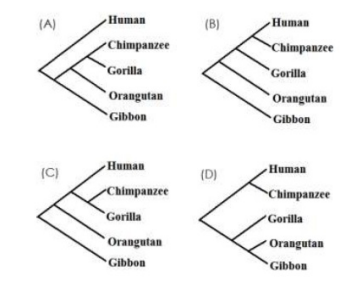
\includegraphics[]{figs/O.21.png}
    \caption{}
    \label{fig:2}
\end{figure}
   
\hfill{(GATE EY 2015)}
%22
\item 
Which of the following processes typically does NOT contribute to increase in genetic variation?

\begin{multicols}{4}
\begin{enumerate}
    
\item Mutation
\item Migration
\item Drift
\item Recombination

    \end{enumerate}
    \end{multicols}
\hfill{(GATE EY 2015)}
%23
\item 
Maximum heterozygosity (in decimal notation, not in fractions or percentage) at a neutral locus with two alleles, given random mating, is 
\underline{\hspace{1.5cm}}


    
\hfill{(GATE EY 2015)}
%24
\item 
A predator encounters a group of 10 prey and kills one of them to feed. The probability of getting killed is the same for all prey individuals. The probability that a given prey is killed by the predator is \underline{\hspace{1.5cm}}

\hfill{(GATE EY 2015)}
%25
\item 
All else being equal, among isolated populations comprising of 10, 100, 500 and 1000 individuals, the impact of random genetic drift is LOWEST in the population with\underline{\hspace{1.5cm}} individuals.



\hfill{(GATE EY 2015)}
%26
\item If the mean of a sample is 4 units and its variance is 16 units, then its coefficient of variation (in decimal notation, not in fractions or percentage) is \underline{\hspace{1.5cm}}


\hfill{(GATE EY 2015)}
%27
\item 
A scientist wants to prove that some birds line their nests with aromatic herbs to protect their chicks against insects that parasitize them. Which of the following experiments will NOT help to investigate this hypothesis?


\begin{enumerate}
    
\item Treating the nests containing aromatic herbs with insecticides
\item Comparing insect parasite load in nests with and without aromatic herbs
\item Comparing the effect of aromatic and non-aromatic herbs on the number of parasites
\item Examining the impact of aromatic herbs on insect parasites under laboratory conditions

    \end{enumerate}
    
\hfill{(GATE EY 2015)}
%28
\item Many cranes are highly endangered and are often raised in captivity in zoos by having wild-collected eggs hatched in incubators. The hatchlings are then reared by the zoo keepers in the absence of adult cranes. In order to ensure successful reproduction of these zoo-reared cranes in the wild, which of the following should NOT occur?

\begin{enumerate}
    
\item Hatchlings must be fed their wild diet by the zoo keepers
\item Hatchlings must be exposed to predators by the zoo keepers
\item Hatchlings should imprint on the zoo keepers
\item Hatchlings should be trained to forage naturally in the wild by the zoo keepers

    \end{enumerate}
    
\hfill{(GATE EY 2015)}
%29
\item Acoustic signals degrade most rapidly in which of the following environments?


\begin{multicols}{2}
\begin{enumerate}
    
\item In a rainforest
\item At a depth of 100 ft in the open ocean
\item In a desert
\item In a Eucalyptus plantation

    \end{enumerate}
    \end{multicols}
\hfill{(GATE EY 2015)}
%30
\item A plant species X is dioecious, another plant species Y is bisexual and cross-pollinated, while a third plant species Z is bisexual and self-pollinated. All else being equal, what might be the expected pollen:ovule ratio when arranged in descending order?


\begin{multicols}{2}
\begin{enumerate}
    
\item$ Y > Z > X$
\item$ X > Y = Z$
\item$ X > Y > Z$
\item $X < Y = Z$

    \end{enumerate}
    \end{multicols}
\hfill{(GATE EY 2015)}
%31
\item 
The nodes of Ranvier are


\begin{enumerate}
    
\item Junctions in connective tissue
\item Myelinated junctions in nerve cells
\item Nodes in sarcolemmas
\item Non-myelinated gaps in nerve cells

    \end{enumerate}
   
\hfill{(GATE EY 2015)}
%32
\item 
Many agriculturally important insect pests belong to which of the following groups?

P) Coleoptera, Q) Odonata, R) Lepidoptera, S) Orthoptera, T) Chiroptera

\begin{multicols}{4}
\begin{enumerate}
    
\item P, Q and S
\item S, R and T
\item Q, S and T
\item P, R and S

    \end{enumerate}
    \end{multicols}
\hfill{(GATE EY 2015)}





%33

\item 

Plasmodesmata are found in
\begin{multicols}{4}
\begin{enumerate}
    
\item Cyanobacteria
\item Plants
\item Invertebrates
\item Vertebrates

    \end{enumerate}
    \end{multicols}
\hfill{(GATE EY 2015)}
%34
\item 
In the schematic below, the circles and triangles represent climatic zones occupied by two different biomes along gradients of precipitation and temperature. Which of the following is an accurate description of these biomes?

\begin{figure}[H]
    \centering
    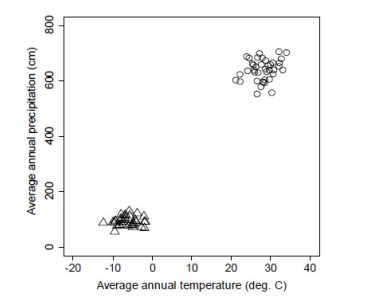
\includegraphics[]{figs/Q.34.png}
    \caption{}
    \label{fig:3}
\end{figure}
\begin{enumerate}
    
\item Circles = Tropical Rainforest; Triangles = Temperate Rainforest
\item Circles = Subtropical Desert; Triangles = Tropical grassland
\item Circles = Tropical Rainforest; Triangles = Tundra
\item Circles = Tundra; Triangles = Subtropical Desert

    \end{enumerate}
    
\hfill{(GATE EY 2015)}

%35
\item 
Flower colour in a plant is governed by a gene with two alleles (A1 and A2). The genotypes A1A1, A2A2 and A1A2 produce red, white and pink flowers, respectively. The frequency of white flowers in a population is 0.16. In an experiment, if only the plants with pink flowers are selfed, then the resulting ratio of red:pink:white phenotypes in the next generation is expected to be

\begin{multicols}{4}
\begin{enumerate}
    
\item 3:2:1
\item 2:2:1
\item 1:2:1
\item 1:1:1

    \end{enumerate}
    \end{multicols}
\hfill{(GATE EY 2015)}

%36
\item 
A researcher studying the effect of urban environment on bird song finds that urban bird song is higher pitched than rural bird song. To test whether this difference has a genetic basis or is due to phenotypic plasticity, she creates four experimental treatments:


\begin{tabular}{|c|c|c|}
\hline
\textbf{Treatment code} & \textbf{Eggs collected from} & \textbf{Eggs hatched and chicks raised in} \\ \hline
RR & Rural & Rural \\ \hline
RU & Rural & Urban \\ \hline
UR & Urban & Rural \\ \hline
UU & Urban & Urban \\ \hline
\end{tabular}



She measures the average pitch of song of adult birds reared from these four treatments and concludes that genetic differences underlie the differences in pitch. Which of the following patterns in the variation in pitch provides evidence for this conclusion?

\begin{multicols}{2}
\begin{enumerate}
    
\item UR = UU = RR = RU
\item$ UU > RU > UR = RR$
\item$ RU > UR > UU = RR$
\item $UR = UU > RR = RU$

    \end{enumerate}
    \end{multicols}
\hfill{(GATE EY 2015)}

%37
\item 
In cooperatively breeding species, a single dominant female breeds while other subordinate adult females in the group rarely breed. Which of the following statements below are PROXIMATE explanations for this phenomenon?
(P) When resources are limited, and competition for reproduction is strong, females evolve costly traits to monopolize reproduction

(Q) Intense aggression by the dominant female towards subordinates results in chronic stress, elevated stress hormone levels, and lowered rates of conception in subordinates

(R) When dispersal is costly, natural selection favours delayed dispersal of the young who instead help rear siblings, in return for continued residence on their natal territory

(S) Pregnant subordinate females are evicted from the group by the dominant female, and harsh conditions outside the group result in loss of body condition and increased risk of abortions
\begin{multicols}{4}
\begin{enumerate}
    
\item P and Q
\item P and R
\item Q and S
\item Q and R

    \end{enumerate}
    \end{multicols}
\hfill{(GATE EY 2015)}


%38
\item 
The figure panels below show population growth in two species (solid circles and open circles), when they are grown alone, and when they are grown together. The interaction between these species is an example of
\begin{figure}[H]
    \centering
    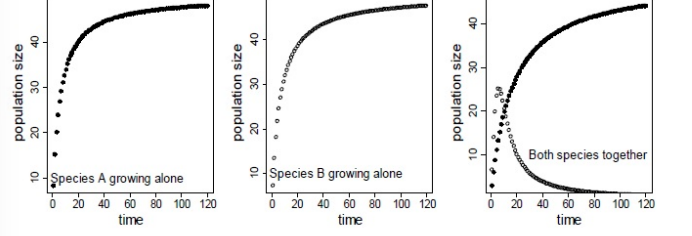
\includegraphics[]{figs/Q.38.png}
    \caption{}
    \label{fig:4}
\end{figure}

\begin{multicols}{2}
\begin{enumerate}
\item mutualism
\item predator-prey interaction
\item competition
\item commensalism

    \end{enumerate}
    \end{multicols}
\hfill{(GATE EY 2015)}



%39

\item In male moths of a certain genus, size of antennae and sensitivity to female pheromone are under the influence of sexual selection. Species X and Species Y of moths within this genus occur together in the same geographical location. Species X naturally occurs in dense populations while Species Y naturally occurs in sparse populations. All else being equal, which of the following is most likely to be correct?



\begin{enumerate}
    
\item  Males of Species X have larger antennae and are more sensitive to female pheromone
\item Males of Species Y have smaller antennae and are less sensitive to female pheromone
\item Males of Species X have smaller antennae and are less sensitive to female pheromone
\item Males of Species Y have larger antennae and are less sensitive to female pheromone



    \end{enumerate}
  
\hfill{(GATE EY 2015)}




%40

\item 
Which of the following figures represents the equation \[y =x^2-c\],where c is a positive constant?


\hfill{(GATE EY 2015)}

\begin{figure}[H]
    \centering
    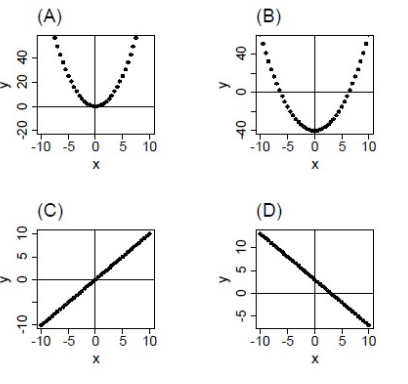
\includegraphics[]{figs/O.40.png}
    \caption{}
    \label{fig:5}
\end{figure}

%41
\item A researcher measures tail length of 1000 individuals in a bird species. In one population, mean tail length $(\pm SD)$ was $15 (\pm 8)$ while it was $10 (\pm 2)$ in a second population, as depicted in the figure below. These values remain consistent across many generations. From these data, he can infer that

\begin{figure}[H]
    \centering
    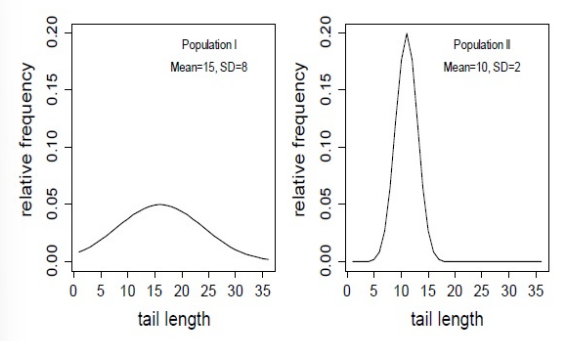
\includegraphics[]{figs/Q.41.png}
    \caption{}
    \label{fig:6}
\end{figure}

\begin{enumerate}
    
\item Population I is under stronger directional selection than population II
\item Population II is under stronger directional selection than population I
\item Population I is under stronger stabilizing selection than population II
\item   Population II is under stronger stabilizing selection than population I

    \end{enumerate}
    
\hfill{(GATE EY 2015)}

%42

\item 
The figure below shows how feeding rate varies with age (old/young) and with body size (small/large) in males of a deer species. Based on this figure, which of the statements below is FALSE?

\begin{figure}[H]
    \centering
    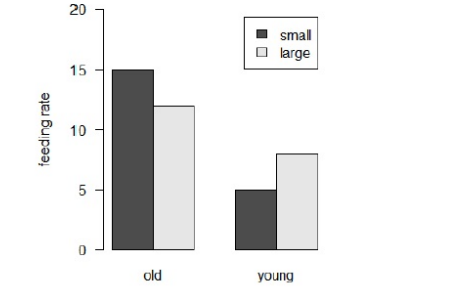
\includegraphics[]{figs/Q.42.png}
    \caption{}
    \label{fig:7}
\end{figure}
\begin{enumerate}
    
\item  Large old males have higher feeding rates than large young males
\item  Large young males have higher feeding rates than small young males
\item  Regardless of size, feeding rate is higher in old males than in young males
\item Regardless of age, feeding rate is higher in small males than in large males

    \end{enumerate}
    
\hfill{(GATE EY 2015)}


%43

\item 
Breeding males in a population show two alternative mating tactics: T1 and T2. These two tactics are hypothesized to be maintained by negative frequency-dependent effects on fitness. Which figure below represents negative frequency-dependence acting on the two tactics?

\begin{figure}[H]
    \centering
    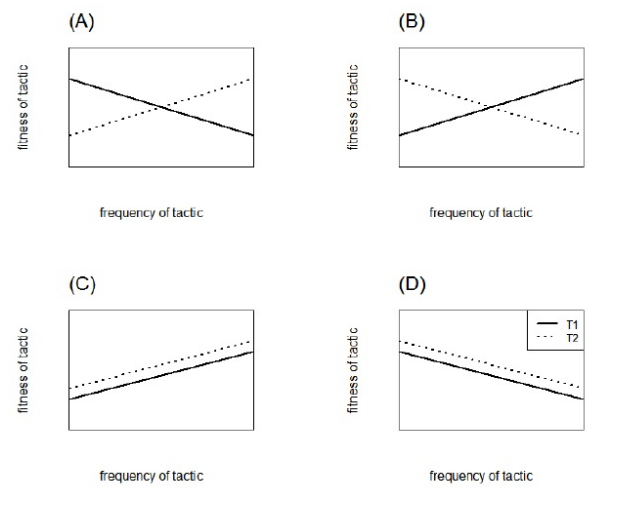
\includegraphics[]{figs/O.43.png}
    \caption{}
    \label{fig:8}
\end{figure}
\hfill{(GATE EY 2015)}


%44



\item 
From an original population P of a butterfly species, two experimental populations X and Y were established. In X, males and females were maintained in standard conditions, and females were allowed to mate and lay eggs. Only eggs from females laying small clutches, i.e., 5 eggs or fewer, were allowed to hatch and the rest were not utilized. In Y, males and females were maintained in standard conditions and females were allowed to mate and lay eggs. From each female, 5 eggs were randomly selected and allowed to hatch, and the rest were not utilized. After 20 generations of these experimental conditions, relative to the original population P, and assuming that clutch size is under genetic control, we expect clutch size to be \underline{\hspace{1.5cm}}  in X and\underline{\hspace{1.5cm}} in Y.

\begin{multicols}{2}
\begin{enumerate}
    
\item  same; same
\item reduced; same
\item same; reduced 
\item reduced; reduced

    \end{enumerate}
    \end{multicols}
\hfill{(GATE EY 2015)}


%45


\item 
Which of the following factors contribute to INCREASING beta diversity of tree species in a typical landscape?

(P) Habitat heterogeneity

(Q) Dispersal limitation

(R) Random mortality among trees

(S) Differences in physiological tolerance among specie
\begin{multicols}{4}
\begin{enumerate}
    
\item  Only P
\item  P and R
\item P, Q and S
\item P, Q, R and S

    \end{enumerate}
    \end{multicols}
\hfill{(GATE EY 2015)}




%46
\item 

The area of a large forest is reduced by 10\% due to fires. Assuming that the number of species (denoted by $S$) and area (denoted by $A$) are related by the equation 
\[ S = cA^z, \]
where $c$ is a positive constant and $z$ is a positive number less than one, the expected loss of species is



\begin{enumerate}
    
\item 10\%
\item more than 10\%
\item less than 10\%
\item cannot be estimated without knowing the exact values of c and z

    \end{enumerate}
    
\hfill{(GATE EY 2015)}


%47

\item The slope of the function   \[y =x-x^2\] at x=1 is \underline{\hspace{1.5cm}}


\hfill{(GATE EY 2015)}
%48


\item 
In which of the following four plots, showing reproductive fitness versus a trait, is the strength of selection MAXIMUM?

\begin{figure}[H]
    \centering
    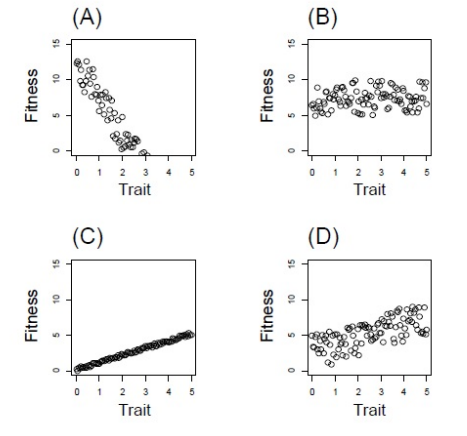
\includegraphics[]{figs/Q.48.png}
    \caption{}
    \label{fig:9}
\end{figure}
\hfill{(GATE EY 2015)}





%49

\item 
Assuming that the chance of a male or female being born is equal, the probability (in decimal notation, not in fractions or percentage) that three out of four offspring born are female is \underline{\hspace{1.5cm}}


\hfill{(GATE EY 2015)}

%50
\item An animal starts moving from point O as shown in the diagram below. At every junction marked by a thick circle, it has an equal probability of choosing any of the paths that takes it northwards.
\begin{figure}[H]
    \centering
    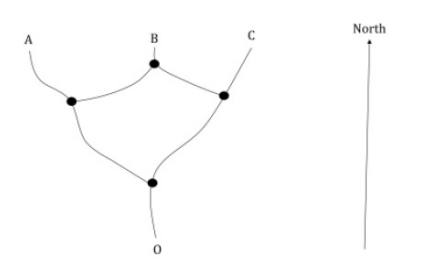
\includegraphics[]{figs/Q.50.png}
    \caption{}
    \label{fig:10}
\end{figure}
\hfill{(GATE EY 2015)}


The probability (in decimal notation, not as fraction or percentage) that the animal will reach point B is \underline{\hspace{1.5cm}}

\hfill{(GATE EY 2015)}


%51
\item 

he Shannon index (H) for diversity is given by 
\[
H = - \sum_i p_i \log_e(p_i)
\]
where $p_i$ is the proportion of species $i$ in the total population.

For the community of species given below, the Shannon index (H) is \underline{\hspace{2cm}}.

\begin{center}
\begin{tabular}{|c|c|}
\hline
\textbf{Species} & \textbf{Population size} \\ \hline
P & 5  \\ \hline
Q & 10 \\ \hline
R & 20 \\ \hline
S & 25 \\ \hline
T & 40 \\ \hline
\end{tabular}
\end{center}



    
\hfill{(GATE EY 2015)}



%52
\item 
n a large forested landscape, where seed dispersal is the ONLY determinant of tree species distribution, two individual trees were randomly picked at a distance r units apart. If F(r) is the probability that the two individuals belong to the same species, which of the following figures shows how F(r) changes with r?

\begin{figure}[H]
    \centering
    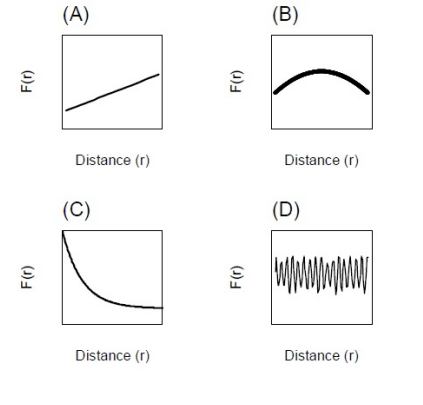
\includegraphics[]{figs/O.52.png}
    \caption{}
    \label{fig:11}
\end{figure}


\hfill{(GATE EY 2015)}

%53

\item 
Bacteria growing exponentially increase in number from 
 $10^{5}$ to $10^{6}$in two hours. The ratio of per capita growth rate at the end of two hours to the per capita growth rate at the initial time is \underline{\hspace{2cm}}


\hfill{(GATE EY 2015)}


%54


\item The figures below represent age-specific survivorship and fecundity for species X (denoted by open circles) and Y (closed circles). Based on these survivorship-fecundity relationships, which of the following can be inferred?
\begin{figure}[H]
    \centering
    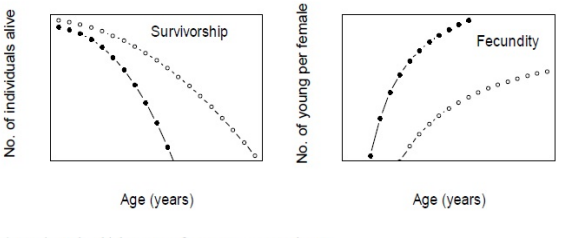
\includegraphics[]{figs/Q.54.png}
    \caption{}
    \label{fig:12}
\end{figure}

(P) Species Y has higher rates of turnover compared to X

(Q) Species Y has a longer life span and delayed reproduction compared to X

(R) Species X has steeper age-specific mortality compared to Y

(S) Species Y is more likely to colonize a site after disturbance compared to X


\begin{multicols}{4}
\begin{enumerate}
    
\item P and S
\item Q and R
\item P, R, and S
\item R and S

    \end{enumerate}
    \end{multicols}
\hfill{(GATE EY 2015)}

%55

\item Tree densities are measured in 5 plots in a study area. An index (Variance in tree density / Mean tree density) estimates whether trees are randomly distributed, clumped, or spaced uniformly apart. Tree densities in these 5 sampled plots were 13, 14, 15, 16, and 17. The value of the above index for this data set is \underline{\hspace{2cm}}

\hfill{(GATE EY 2015)}
%56


\item 
The ratio of Potential Evapotranspiration (PET) to Precipitation (PT) is expected to be more than 1, i.e., PET/PT $>$ 1, in which of the following biomes?

\begin{multicols}{4}
\begin{enumerate}
    
\item Tropical rainforest
\item Arid grassland
\item Tundra 
\item Taiga

    \end{enumerate}
    \end{multicols}
\hfill{(GATE EY 2015)}


%57

\item 
Redox potential (Eh) indicates the capacity of atoms, ions, or molecules to donate or accept electrons (i.e., electric potential of energetic transformation during chemical reactions). For reactions involving the nitrogen cycle, Eh values are the following %there is a table

A consequence of these differences is that:



\begin{center}
\begin{tabular}{|c|c|}
\hline
\textbf{Reaction} & \textbf{Eh (volts)} \\ \hline
$\mathrm{NO_3^- \ to \ N_2}$ & +0.75 \\ \hline
$\mathrm{NO_3^- \ to \ NO_2^-}$ & +0.42 \\ \hline
$\mathrm{NO_2^- \ to \ NH_4^+}$ & +0.34 \\ \hline
$\mathrm{N_2 \ to \ NH_4^+}$ & -0.28 \\ \hline
\end{tabular}
\end{center}
\begin{enumerate}
\item N-fixation is energetically unfavourable
\item Denitrification is energetically unfavourable 
\item Both N-fixation and denitrification are energetically favourable
\item Both N-fixation and denitrification are energetically unfavourable

    \end{enumerate}
    
\hfill{(GATE EY 2015)}


%58

\item A bird has the choice of four food resources with the following characteristics:
\begin{center}
\begin{tabular}{|c|c|p{5cm}|}
\hline
\textbf{Resource} & \textbf{Energy content (cal/g)} & \textbf{Energy expended in  searching for and handling the resource (cal/g)} \\ \hline
P & 20 & 30 \\ \hline
Q & 85 & 30 \\ \hline
R & 65 & 20 \\ \hline
S & 90 & 15 \\ \hline
\end{tabular}
\end{center}
Assuming that all resources are equally abundant and that the bird forages for these resources in an optimal manner, it should exhibit the following sequence of preferences for the resources


\begin{enumerate}
 \item $S>Q>R>P$
 \item $Q>S>R>P$
 \item $S>R>Q>P$
 \item $S>R>Q=P$
   \end{enumerate}
    
\hfill{(GATE EY 2015)}


%59
\item 
A scientist conducts an experiment to test the ability of the worm Caenorhabditis elegans to find a food source using only its odour. She places only food odour in the left arm of a Y-shaped tube; there is no food odour in the right arm. She tests 50 worms individually in separate tubes. She finds that they all move into the left arm. She concludes that individual worms can find food using odour alone. However, another scientist says that the experiment is flawed. Based on the information provided above, which of the following is a valid objection?


\begin{enumerate}
    
\item Worms could have used vision to find the food source
\item Worms should have also been tested with the odour placed in the right arm
\item Worms should all have been tested together in the same tube
\item  Worms should have been tested individually using the same tube

    \end{enumerate}
    
\hfill{(GATE EY 2015)}



%60
\item
The DNA sequence -AAAAAAAAAAAA- undergoes substitutions at the rate of one change every day. Assuming that all base changes are equally probable, the MOST LIKELY composition of this 12 base pair sequence at the end of ten years will be
 

\begin{multicols}{2}
\begin{enumerate}
    
\item A=0.25 T=0.25 G=0.25 C=0.25
\item A=0.75 T=0.15 G=0.05 C=0.05 
\item A=0.70 T=0.10 G=0.10 C=0.10
\item A=0.40 T=0.40 G=0.10 C=0.10

    \end{enumerate}
    \end{multicols}
\hfill{(GATE EY 2015)}


%61

\item 
There is a tightly-linked association between host and symbiont in obligate mutualisms; for example, between termites and their gut symbionts. The following is the phylogeny of the host species A, B, C, D and E, which harbour symbionts Sa, Sb, Sc, Sd and Se.
\begin{figure}[H]
    \centering
    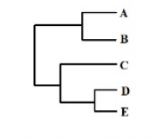
\includegraphics[]{figs/Q.61.png}
    \caption{}
    \label{fig:13}
\end{figure}
Assuming obligate mutualism between these hosts and symbionts, the phylogeny of the symbionts is best represented by which of the following trees?

\begin{figure}[H]
    \centering
    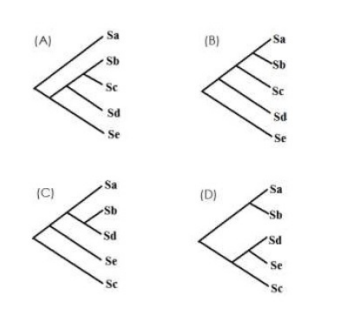
\includegraphics[]{figs/O.61.png}
    \caption{}
    \label{fig:14}
\end{figure}


\hfill{(GATE EY 2015)}


%62

\item 
Anita wants to study the effect of Compound X on leaf expansion rates in 100 individuals of a plant species S. Which of the following constitute suitable control(s) for this experiment?

P) Simultaneously measure leaf expansion rates in a second set of 100 plants of species S which has not been treated with Compound X.
Q) Measure leaf expansion rates in a second set of 100 plants of species S which has been treated with Compound X for a longer duration.
R) Measure leaf expansion rates in a set of 100 plants belonging to a different but closely related plant species treated with Compound X.
S) Measure leaf expansion rates for a second set of 100 plants of species S treated with Compound X to test for repeatability of results.

\begin{multicols}{4}
\begin{enumerate}
    
\item P only
\item Q and S
\item R only
\item P and S

    \end{enumerate}
    \end{multicols}
\hfill{(GATE EY 2015)}

%63


\item 
Three sanctuaries X, Y and Z have the same number of mammal species but different species compositions. The list of mammals reported from these sanctuaries is given below.

Sanctuary X : Langur, tiger, spotted deer, leopard, bison, wild dog, elephant
Sanctuary Y : Lion, spotted deer, leopard, hyena, langur, blackbuck, wild boar
Sanctuary Z : Gibbon, tiger, spotted deer, leopard, bison, rhinoceros, elephant

Which of the following options best describes the order-level diversity in these sanctuaries?

\begin{multicols}{4}
\begin{enumerate}
    
\item $X=Y=Z$
\item $X>Y=Z$
\item $X=Y>Z$
\item $X\not=Y\not=Z$

    \end{enumerate}
    \end{multicols}
\hfill{(GATE EY 2015)}




%64

\item 
The evolutionary relationship between five species of birds (A to E) is shown below.
\begin{figure}[H]
    \centering
    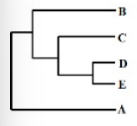
\includegraphics[]{figs/Q.64.png}
    \caption{}
    \label{fig:15}
\end{figure}

Species C, D, and E have a crest while the rest do not. Given this phylogeny and the principle of parsimony (i.e., involving the fewest number of evolutionary steps), which of the following statements reflects the evolution of the crest in this group?

\begin{enumerate}
    
\item  Crests evolved multiple times in this group
\item The common ancestor of the five species did not have a crest
\item Species B and A lost their crests in the course of evolution
\item The presence of a crest in species C, D and E is due to convergence

    \end{enumerate}
    
\hfill{(GATE EY 2015)}


%65


\item 
Parental care may be provided by only males, only females, or by both parents. Comparing parental care between mammals, birds and fishes, male-only care is most common in  female-only care is most common in  \underline{\hspace{2cm}} and biparental care is most common in  \underline{\hspace{2cm}} 
\begin{multicols}{2}
\begin{enumerate}
    
\item  birds; fishes; mammals
\item fishes; birds; mammals
\item birds; mammals; fishes
\item fishes; mammals; birds
    \end{enumerate}
    \end{multicols}
\hfill{(GATE EY 2015)}




\end{enumerate}
\end{document}